% Number 850
% CAPMA Algebra Units 
% Hot air balloon camera drop
% JG

% Watermark
\AddToShipoutPicture*{\BackgroundPic}

\addtocounter {ProbNum} {1}

%\begin{floatingfigure}[r]{.44\textwidth}
%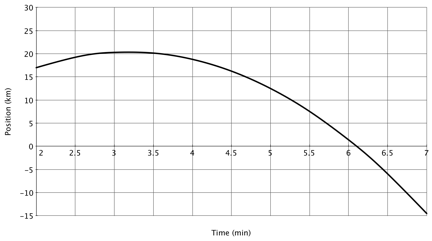
\includegraphics[scale=.5]{/Users/jgates/desktop/latex/pics/xgraph2}
%\end{floatingfigure}
 
{\bf \Large{\arabic{ProbNum}}} A hot-air balloon is 45 meters off of the ground, ascending at a rate of 2 meters per second, when the pilot drops (releases) his camera.  \bigskip

How long will it take to hit the ground?\paragraph{}
\noindent
\vfill


%\begin{center}
%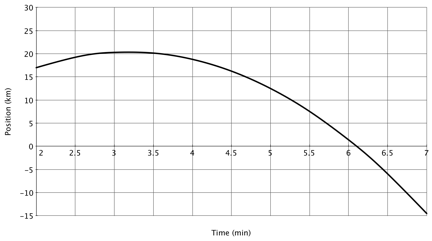
\includegraphics[scale=1]{/Users/jgates/desktop/latex/pics/xgraph2}
%\end{center}


\newpage